\chapter{Correlative Analysis}

The chapter looks at some of the fundamentals of correlative analysis for dynamic systems, and discusses the merits and demerits of various correlative methods.

\section{Correlation for Fault Analysis: Motivation}

In Chapter 2, we discussed some of the common methods for FDIR on complex systems, using linear system models that represent system state in terms of directly or indirectly telemetered values. However, there is key information that such an analysis can miss: the underlying connections between different telemetry channels. These connections can suggest semantic links, and even causations, between properties of the system, and can thus be used to link identified faults with unidentified changes of significance in other telemetered values. As such, a thorough study of the correlative attributes of a system can provide a framework with which its internal structure may be examined, and may even suggest modes of operation which can be used to understand higher-level system behavior.

\subsection{Covariance Matrices}

Covariance is defined as a measurement of the strength of correlation between two or more sets of random variables; i.e., it shows how much these variables ``change together." Statistically, for two variables $x$ and $y$, the covariance is the expected value of the product of the standard deviations of each of the variables:
\begin{equation} \label{eq:cov}
\mathrm{cov} = \text{E}[(x - \mu_{x})(y - \mu_{y})]
\end{equation}

Intuitively, it can be seen that a situation in which $x$ and $y$ both are much larger (or both much smaller) than their respective means results in a high covariance; a situation where $x$ is much larger than its mean, but $y$ is around its mean, will result in a small covariance. In this way, the correlation between these two variables is captured by a covariance measurement.

For a vector of random variables $\bar{x} \in \mathbb{R}^{n}$, there exists a symmetric covariance matrix $\Sigma \in \mathbb{R}^{n \times n}$ such that $\Sigma_{ij}$ is the covariance between $\bar{x}_{i}$ and $\bar{x}_{j}$. This matrix captures valuable correlative data about the system.

When looking at two sets of data, it can often be valuable to reduce their interdependence (i.e., how much they change in sync with each other) into a single number, or ``correlation coefficient." This coefficient is often a more generic version of the covariance, such that it can be used as straightforward metric to determine correlation between sets of times series data. It may even be used as input into visualization algorithms to affect shading or even positioning, as we will see in later chapters.

\subsection{Pearson Correlation Coefficient}

The Pearson Correlation Coefficient (PCC), also known as the Pearson Product-Moment Coefficient, is a metric of the linear relationship between two sets of data. It is essentially a scaled covariance, defined as \\
\begin{equation} \label{eq:pcc}
\text{PCC}_{X, Y} = \frac{\mathrm{cov}(X, Y)}{\sigma_{X} \sigma_{Y}}
\end{equation}

where $X$ and $Y$ are two vectors of data (or, in the case of the telemetry data sets we examine in this paper, times series of values over time for two telemetry channels). The PCC gives a quantified measurement of the linear correlation between the two vectors, in the form of a value in the range of $[-1, 1]$, where $1$ is a total positive correlation, $-1$ is a total negative correlation, and $0$ is no correlation at all.

The Pearson Correlation Coefficient carries with it a few important assumptions:

\begin{itemize}
\item Samples have values that are interval or ratio variables (not ordinal or categorical).
\item Sample pairs have a linear relationship (or, at least, these are the type of relationships you wish to see).
\item Sample pairs follow a bivariate normal distribution.
\end{itemize}

If the data doesn't fit the assumptions above, one of the two rank correlation coefficients discussed below may be more appropriate. In many of the spacecraft telemetry datasets we may encounter, the latter two assumptions will not hold, so the rank correlation coefficients will be of greater use.

\subsection{Spearman Rank Correlation Coefficient ($\rho$)}

The Spearman Rank Correlation Coefficient, or ``Spearman's Rho," is a type of correlation coefficient, which, like the PCC, seeks to quantify relationships between vectors of data, but which looks the ranking of variables within an ordering, rather than their linear relationship. This allows the coefficient to express relationship \textit{monotonicity}, in order to be less dependent on linearity of relationships. It actually makes uses of the PCC to do this, by calculating the PCC on the ranked data values.

Spearman's Rho is calculated by ranking the values for each variable, and then performing this calculation on those ranks:
\begin{equation} \label{eq:rho}
\rho_{X, Y} = 1 - \frac{6 \sum{d_{i}^{2}}}{n(n^{2}-1)},
\end{equation}

where $d_{i}$ is the difference in paired ranks, and $n$ is the number of observations. Like the PCC, Spearman's Rho takes the form of a value in the range of $[-1, 1]$, where $1$ is a total positive correlation, $-1$ is a total negative correlation, and $0$ is no correlation at all.

Spearman's Rho has assumptions which are far less restrictive than those of the PCC \cite{spearmans}:

\begin{itemize}
\item Samples have values that are interval, ratio or ordinal variables (not categorical).
\item Sample pairs must have a monotonic relationship (or, at least, these are the type of relationships you wish to see).
\end{itemize}

These relaxed assumptions allow for its confident application to a wider variety of real system data.

\subsection{Kendall Rank Correlation Coefficient ($\tau$)}

The Kendall Rank Correlation Coefficient, like ``Spearman's Rho," seeks to capture non-linear dependence by using the ordered ranks of the argument variables as input to the algorithm.

Kendall's Tau is defined as follows:
\begin{equation} \label{eq:tau}
\tau_{X, Y} = \frac{n_{c} - n_{d}}{n(n^{2}-1)/2},
\end{equation}

where $n_{c}$ is the number of ``concordant pairs" (pairs of variables with the same rank order across observations), $n_{d}$ is the number of ``discordant pairs" (pairs of variables with different rank order across observations), and $n$ is the number of observations.

Kendall's Tau carries with it the same assumptions as Spearman's Rho \cite{kendalls2}.

\section{Limitations of Traditional Correlative Techniques}

There are many limitations to the three traditional correlative techniques above, and it's important to understand them, even if the ultimate decision will be to use one of these techniques. Some of the major limitations are decribed below.

\subsection{Linearity Assumptions}

As discussed above, the PCC algorithm assumes that correlated data has a linear relationship between variables, and cannot adequately model nonlinear relationships. Many dynamic relationships that may be telemetered on a complex system are nonlinear, and will not be properly modeled using PCC. In contrast, the rank correlation methods model in terms of monotonicity, so they can capture many associative relationships that PCC cannot. Certain specially crafted pathological data sets can successfully confound PCC while being intuitively represented by rank correlation methods; see \cite{anscombe1973graphs} for the classic example of ``Anscombe's Quartet."

% \subsection{Multivariate Normal Distances vs. Elliptical Distances}

\subsection{Implied Causation}

One caveat of which a human operator must always be aware, especially when trying to build intuition and make conclusions based on correlative data, is that the formulations of correlation described above do not imply causation, and causation should not be inferred simply due to a high correlation score. However, correlation may \textit{suggest} causation, and can provide valuable next steps for data examination informed by expert knowledge.

\begin{figure}[h]
\centering
    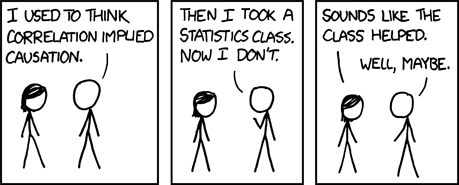
\includegraphics[width=0.5\columnwidth]{images/xkcd_correlation.png}
    \caption{A comical observation on the nature of correlation and causation. From \cite{xkcd_correlation}.}
    \label{fig:xkcd_correction}
\end{figure}

% \subsection{Alternatives to Correlation Score Techniques}

% \subsection{Applications of Correlation to Residual-Based Fault Analysis}

% Though we will be primarily examining the use of correlation for data discovery and root cause diagnosis, it's worth noting that correlation state data has been successfully used in previous research to create fault detection residuals to detect an understood fault state. In \cite{isermann1984process}, Isermann 

% Isermann paper

% Discussion of how this is using correlation between telemetry values to look for an understood fault state, rather than for data discovery (but it's still valuable!)



% \subsection{Distance Correlation}

% \subsection{Correlation Ratio}

% \subsection{Brownian Covariance}

% \subsection{Coefficient of Determination}

% \subsection{Polychloric Correlation}